\documentclass{article}
\usepackage[utf8]{inputenc}
\usepackage{titling}
\setlength{\droptitle}{-3cm}
\usepackage[left=2cm,right=2cm,top=3cm,bottom=2cm]{geometry}

\title{2T201 Projet 1\\chaier des charges}
\author{Dourov Maxime, Cruquenaire Achille, Gendebien Jonas}
\date{Octobre 2022}
\newcommand{\HRule}{\rule{\linewidth}{0.5mm}}

\usepackage{tabularx}
\usepackage{amssymb}
\usepackage{graphicx}
\usepackage{booktabs}
\usepackage{caption}
\usepackage{geometry}
\usepackage{float}
\graphicspath{ {./images/} }

\begin{document}

\maketitle
\section{Introduction}
    jean r'prendraisbyunune, étudiant en sociologie,
    désire un jeux de réflexion pour jouer avec ses co-koteurs, basé sur le jeux de dame.
    

\section{Objectifs}
L'objectif du projet est de produire un jeux de dame révisé avec de nouvelles mécaniques.(voir \ref{new_rules})\\
Le jeux doit accommoder au minimum deux joueurs en local et garder un historique des scores, avec un leaderboard des meilleurs joueurs.\\
il a été convenu que l'application utiliserait une interface graphique. l'utilisateur déplacera ces pions avec la souris. Les cases autorisée seront en sur brillance, ainsi que les pion adverse prenable.

\section{Contraintes}
\subsection{Règles standard conservées}
- les pions ne peuvent se déplacer que d'une case en diagonale, vers l'avant\\
- les pions peuvent prendre d'autres pièces en avant \textit{et} en arrière\\
- les pions qui atteignent le 'mur' adverse sont promus en dames\\
- les dames peuvent se déplacer d'un nombre illimité de cases

\subsection{Règles rajoutées ou modifiées}\label{new_rules}
\subsubsection{le plateau est composé d'hexagones}
ce qui implique qu'il ne s'agit plus d'un damier. les position initiales des pions sont donc modifiée (voir image). Il faut également prendre en compte que désormais toutes les cases du plateau sont accessibles; mais un pion seul ne peut pas.\\\\
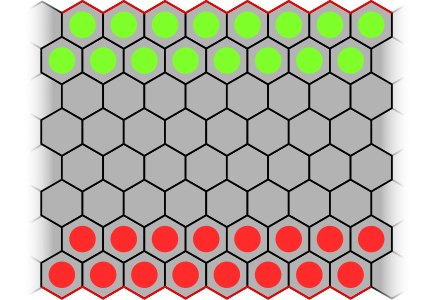
\includegraphics[]{images/normal.png}\label{fig:normal}\\
\newpage
\subsubsection{il y a plus de diagonales possibles pour chaque déplacement}
lors d'une patrie normale un pion ne peut bouger que dans 4 directions, dont deux sont limitée aux prises. alors qu'ici, il y a 5 directions de mouvement (on ne compte pas l'arrière voir\ref{fig:mvt}et\ref{fig:prise})
dans le sens horizontal, le plateau est courbé sur lui même. Donc, en avançant vers le bord vertical du plateau les pièces se retrouvent de l'autre côté.\\\\
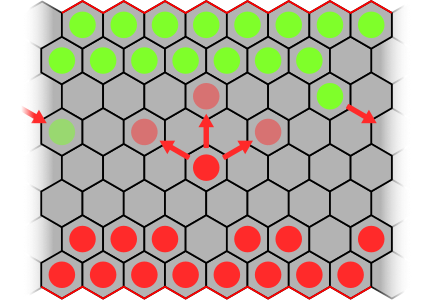
\includegraphics[]{images/mvt.png}\label{fig:mvt}\\
\\
\subsubsection{un pion peut prendre jusqu'à deux pions en un déplacement}
comme l'axe de mouvement choisit n'intercepte pas directement une pièce, nous avons choisit de nous inspirer de la prise en passant des échecs. lors de son déplacement une pièce capturera donc toutes pièce a coté de laquelle elle passe.\\\\
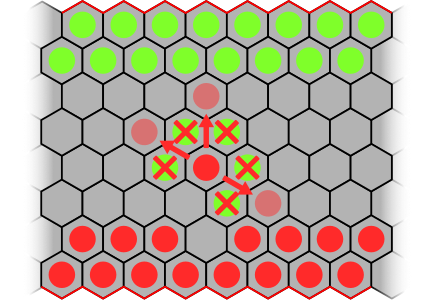
\includegraphics[]{images/prise.png}\label{fig:prise}

\section{Équilibrage}
Comme toutes modification d'un jeux existant peut perturber l'équilibre du jeu, des séance de test (tant en interne qu'avec le client) seront nécessaire pour équilibrer les différentes mécaniques.\\\\
\textbf{Quelques notions qui seront soumises à l'équilibrage:}\\
\subsection{la taille du plateau (départ 8X8):}
nous anticipons que la modification du plateau vers des hexagones perturbera la vitesse de jeu. le plateau sera réduit au grandit en fonction du feedback.
\subsection{les déplacement:}
ors du changement de plateau, un choix concernant le déplacement des pièces à été fait mais il existe deux possibilités.\\
la première est celle utilisée, à savoir les pions suivent les ligne de diagonale jusque a la case suivante. ils prennent les pions à-côté desquels ils passent (voir \ref{fig:prise}).\\
la seconde est de passer de case en case "normalement". la prise sera donc identique au dames classique, soit le pion passe au dessus de la pièce qu'il prend.
\newpage
\subsection{les grilles parallèles:}
il apparais que le jeu tel quel se compose en fait de trois grilles imbriquée. ce qui avec les règles actuelles empêche toute prise entre deux pièce qui ont démarré sur la même grille. il est donc possible de finir une partie sur un match nul. Dans l'image, les trois grilles dans des couleurs différantes.\\\\
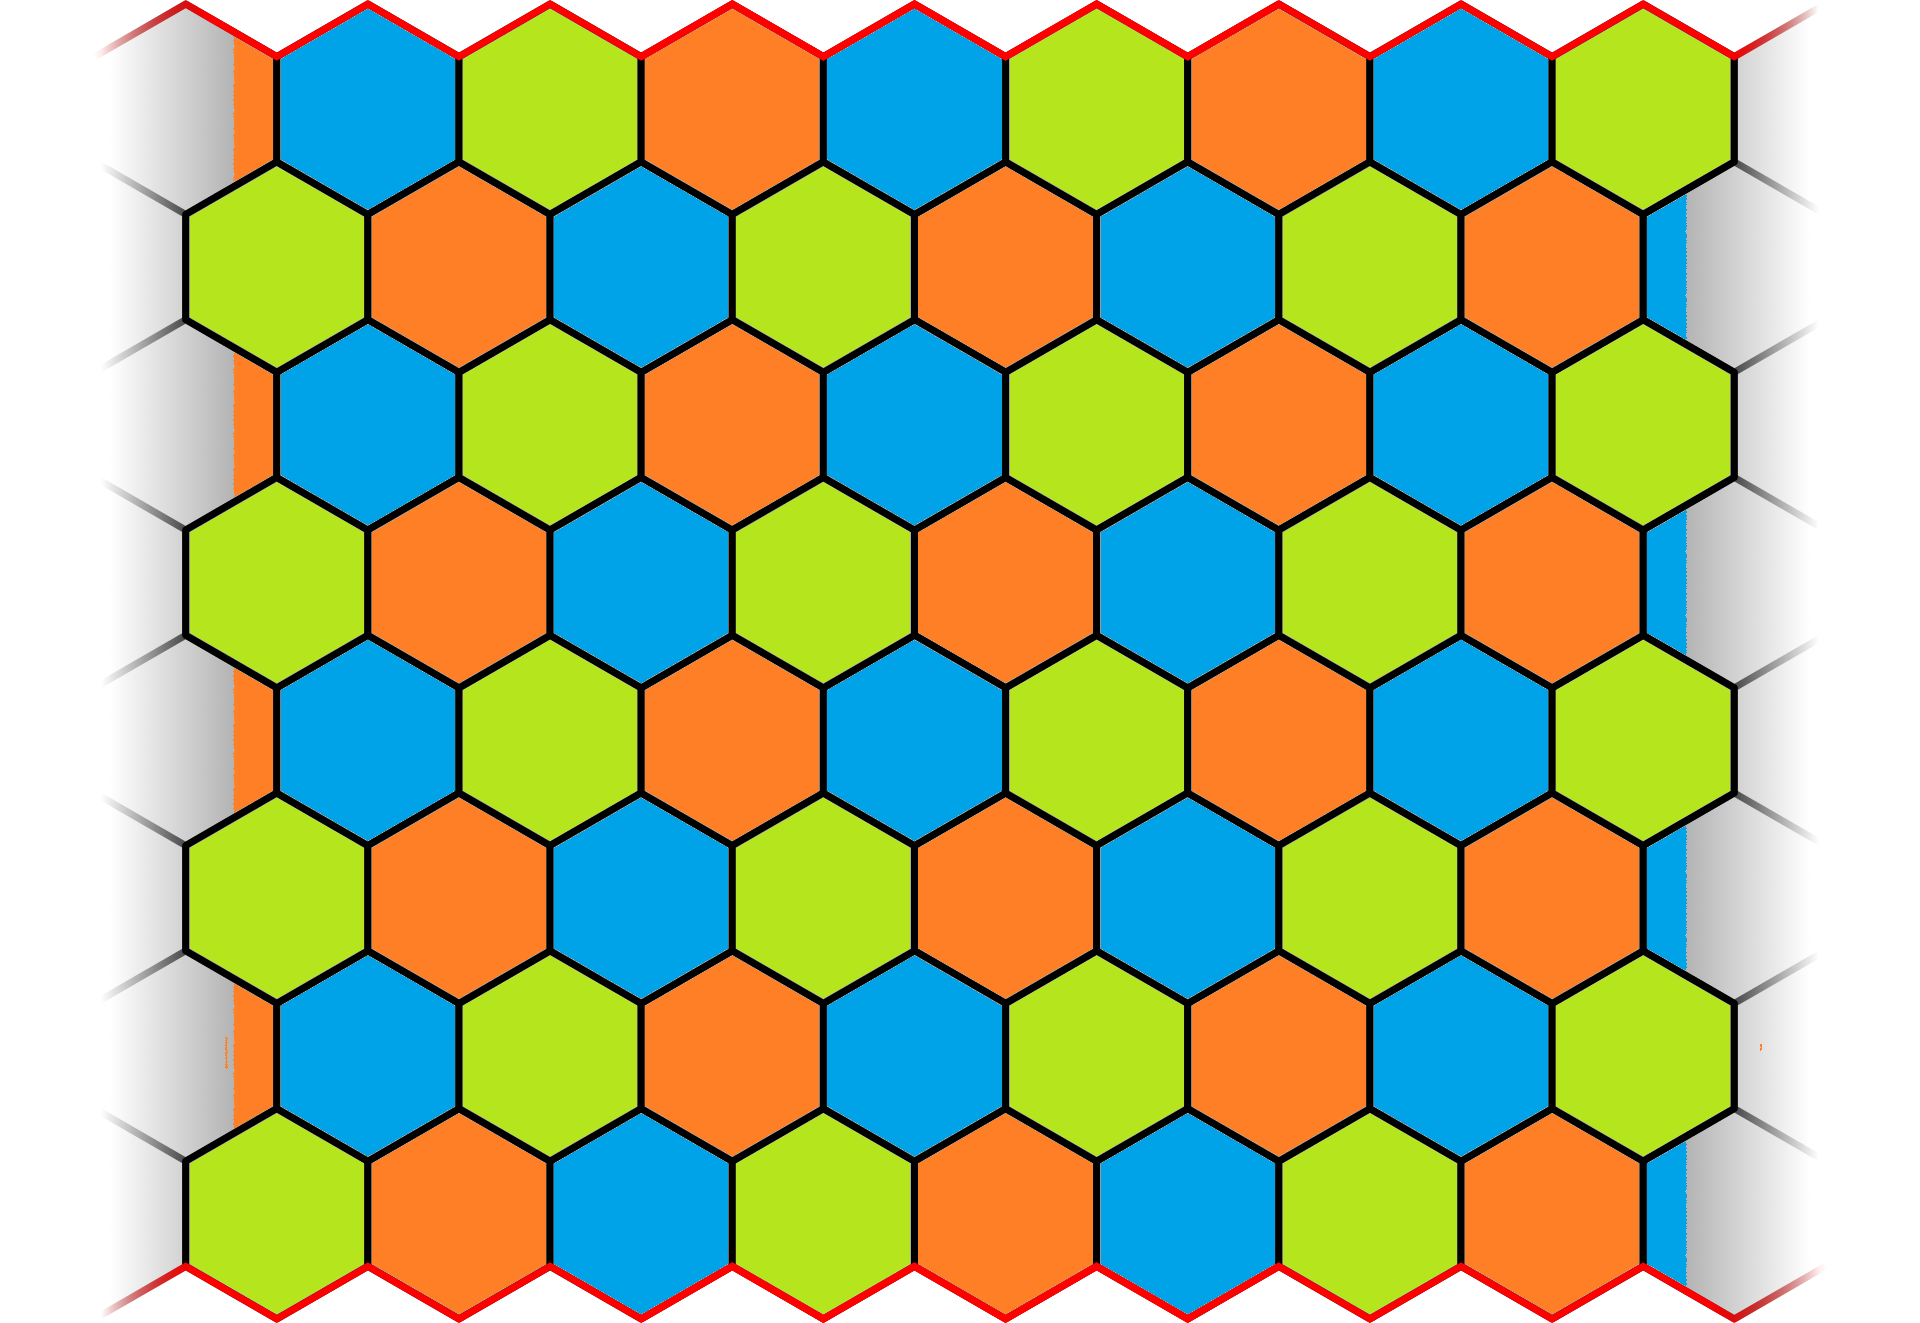
\includegraphics[scale=0.2]{images/board-grids.png}

\section{Planning}
\begin{table}[h]
\begin{tabularx}{\textwidth}{XXXX}
\toprule
\textbf{semaine 1} & \textbf{semaine 2} & \textbf{semaine 3-4} & \textbf{semaine 5-6}\\
\midrule
cahier des charges & prototype graphique & logique partie 1 & logique partie 2 \\ 
\hline
/ & / & prise des pions, changement de joueurs, tour de plateau & leaderboard, fin de partie, dames\\
\bottomrule
\end{tabularx}
\end{table}
Il a été convenu de se réunir toutes les 3 semaines avec le client (les jeudi) pour faire le point des avancée avec le client\\\\
Le projet devra être terminé dans son intégralité pour le 16 décembre

\section{Prototype}
Le MVP sera une démonstration graphique du projet, il permettra de démontrer les mouvements possibles dans le plateau et ne contiendra pas encore les règles du jeu de dames permettant de prendre les pions et garder les scores.

\section{fonctionalitée}
\begin{enumerate}
    \item cases hexagonales
    \item au lancement de l'application, il y a un menu qui permet de choisir entre lancer une partie et afficher le leaderboard
    \item à la fin d'une partie le joueur peut afficher le leaderboard ou relancer une partie
    \item permet à deux joueurs de jouer tour à tour
    \item permet de jouer seul contre l'ordinateur
    \item l'application se souvient des scores précédents
    \item les joueurs choisissent leur nom pour le leaderboard
    \item le plateau est continu horizontalement (voir \ref{new_rules})
    \item les pions arrivant au bout opposé du plateau sont promus en dame
    \item le joueur qui élimine tout les pions adverses gagne
    \item un score est donné à chaque joueur en fonction de leur performances
    \item le gagnant obtient un bonus de points
\end{enumerate}

\section{Budget}
le client dans sa grande générosité s'engage à payer pour les services de développement en visibilité.
les frais horaire de l'équipe sont les suivant:
\begin{table}[h]
    \begin{tabular}{c|c}
    \toprule
        Nom & Honoraires \\
    \midrule
        Cruquenaire Achille &  \\
        Dourov Maxime & \\
        Gendebien Jonas & \\
    \bottomrule
    \end{tabular}
\end{table}\\
---TBD--- estimation du temps de travail 250h? 300?
il faut tenir compte des test et de l'équilibrage

\end{document}